Die Aufgabe dieser �bung bestand darin, einen IIR Filter zu realisieren. Dabei sind folgende Pol- und Nullstellen vorgegeben:
    \centering
    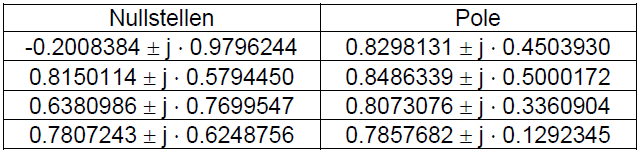
\includegraphics[width=\textwidth]{PolUndNullstellenIIR.png}
Diese haben wir zun\"achst in der z-Ebene gezeichnet, um die Pole und Nullstellen zu Teilsystemen zu kombinieren. 
Dabei waren die 3 Regeln aus der Aufgabenstellung zu beachten.
    \centering
    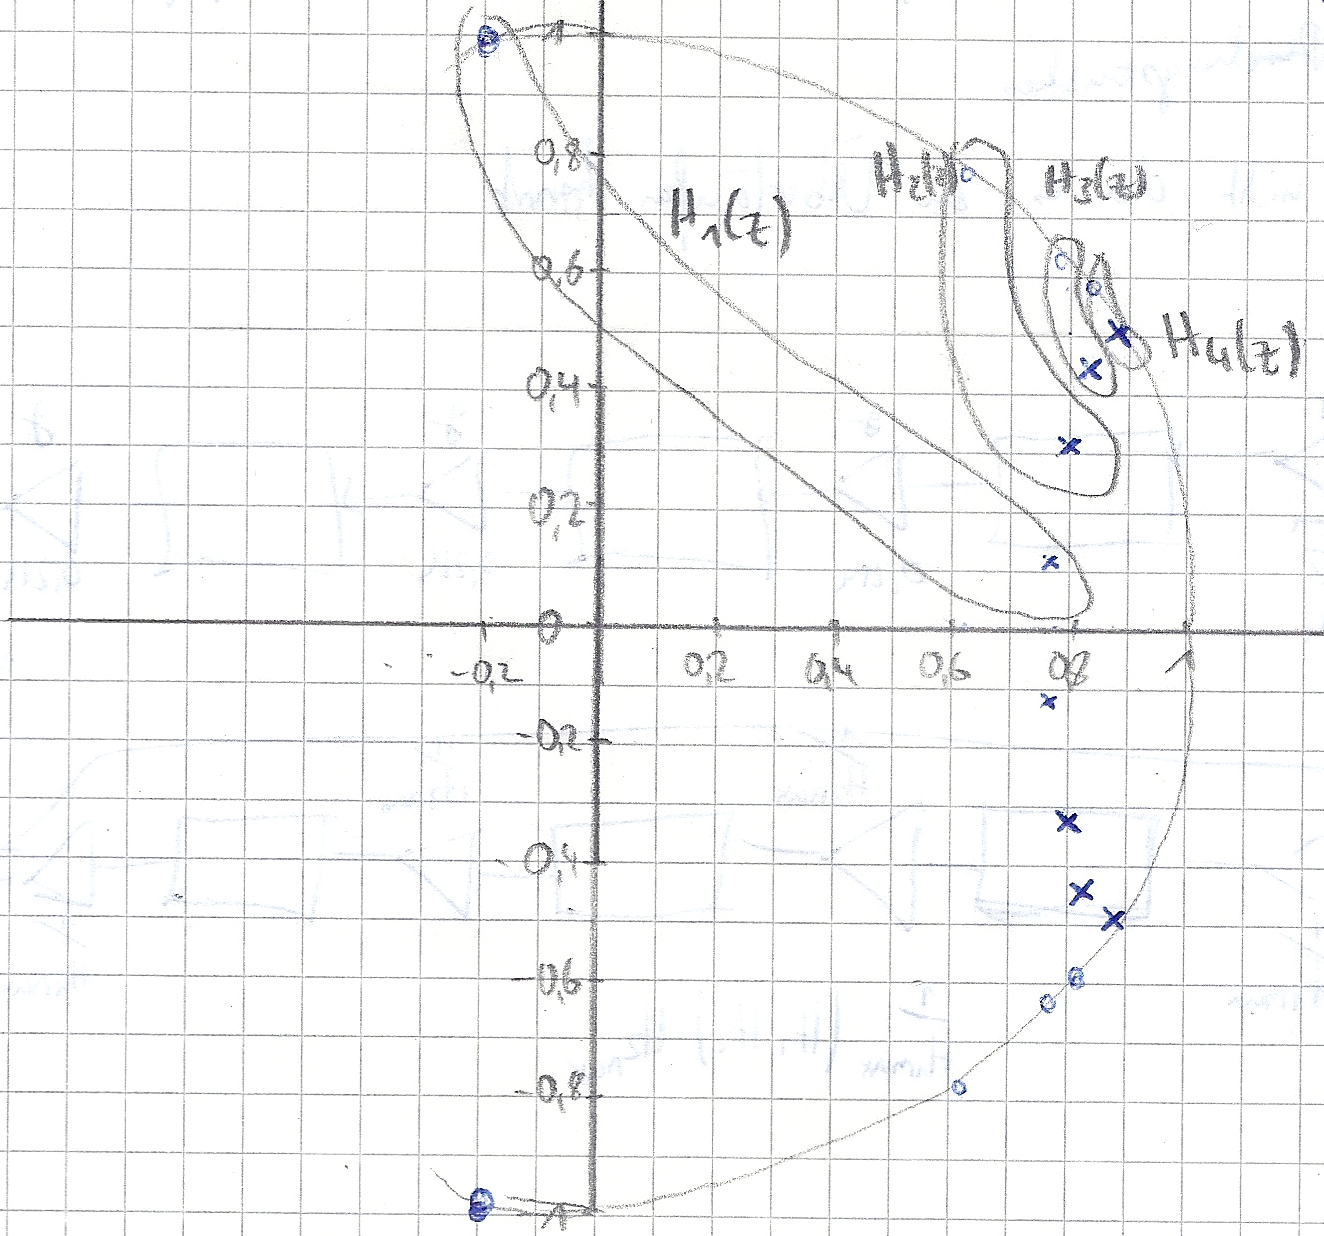
\includegraphics[width=\textwidth]{TeilsystemeZEbene.png}
    \caption{Kombinierte Pol- und Nullstellen}
    \label{fig:PolesAndZeros}
Nun haben wir die \"Ubertragungsfunktionen der 4 Teilsysteme aufgestellt in dem wir die kombinierten Pol- und Nullstellen in folgende Formel einsetzten.
    \centering
    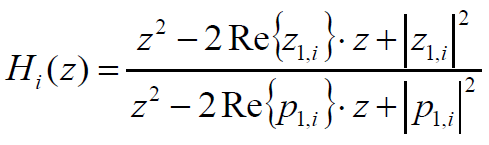
\includegraphics[width=\textwidth]{UeertragungsfunktionFormel.png}
Damit ergeben sich folgende \"Ubertragungsfunktionen:
\begin{equation}
  H_1(z)=\frac{1-1,6300228z^-1+1,00000009z^-2}{1-1,6972678z^-1+0,97019670z^-2}
  H_2(z)=\frac{1-1,5614486z^-1+0,99999995z^-2}{1-1,6596262z^-1+0,89144364z^-2}
  H_3(z)=\frac{1-1,2761982z^-1+1,00000006z^-2}{1-1,6146152z^-1+0,76470231z^-2}
  H_4(z)=\frac{1+0,4016768z^-1+1,00000003z^-2}{1-1,5715364z^-1+0,63413322z^-2}
\end{equation}

Nun war die Durchlassverst\"arkung des Gesamtsystems (ohne Verst\"rkungsfaktor g) f�r die Frequenz f=0 zu berechnen.
Bei einer Frequenz von 0Hz wird z zu 1. Damit lassen sich die Durchlassverst\"arkungen der Teilsysteme aussrechnen. Durch Multplikation dieser erhalten wir
die Durchlassverst\"arkung des Gesamtsystems.
\begin{equation}
  H_1(1)=1,3558
  H_2(1)=1,8921
  H_3(1)=4,8221
  H_4(1)=38,3655
  \Pi H_i(1)=38,3655*4,8221*1,8921*1,3558=474.5917
\end{equation}
Der Kehrwert der Gesamtverst\"arkung ergibt den Faktor mit dem das Gesamtsystem multipliziert werden muss damit die Durchlassverst\"arkung zu 1 wird.
